% Set up the document
\documentclass{article}

% Page size
\usepackage[
    letterpaper,]{geometry}

% Lines between paragraphs
\setlength{\parskip}{\baselineskip}
\setlength{\parindent}{0pt}

% Math
\usepackage{mathtools}
\usepackage{amssymb}
\usepackage{amsthm}
\usepackage{commath}

% Number sets
\newcommand{\C}{\mathbb{C}}
\newcommand{\N}{\mathbb{N}}
\newcommand{\Q}{\mathbb{Q}}
\newcommand{\R}{\mathbb{R}}
\newcommand{\Z}{\mathbb{Z}}

% Links
\usepackage{hyperref}

% Page numbers at top right
\usepackage{fancyhdr}
\pagestyle{fancy}
\fancyhf{}
\fancyhead[R]{\thepage}
\renewcommand\headrulewidth{0pt}

% Graphics
\usepackage{float}
\usepackage{graphicx}
\graphicspath{ {./img/} }

\begin{document}

\textbf{MATH 461 assignment 5} \\
\textbf{Matt Wiens \#301294492} \\
\textbf{2020-07-31}

3.9.14. Write down a differential equation for the following pathway:
%
\begin{equation*}
    A \xrightleftharpoons[k_1]{k_{-1}}
    B \xrightleftharpoons[k_2]{k_{-2}}
    C \xrightleftharpoons[k_3]{k_{-3}}
    A
    .
\end{equation*}

\textit{Solution.}
For this pathway we have the following system of differential equations:
%
\begin{align*}
    \dod{a}{t} &= - k_{-1} a + k_1 b + k_{-3} c - k_3 a
    , \\
    \dod{b}{t} &= k_{-1} a - k_1 b - k_{-2} b + k_2 c
    , \\
    \dod{c}{t} &= k_{-2} b - k_2 c - k_{-3} c + k_3 a
    ,
\end{align*}
%
where $a$, $b$, and $c$, denote the concentrations of A, B, and C, respectively.
Combining terms, we can equivalently write the system as
%
\begin{align*}
    \dod{a}{t} &= - (k_{-1} + k_3) a + k_1 b + k_{-3} c
    , \\
    \dod{b}{t} &= k_{-1} a - (k_1 + k_{-2}) b + k_2 c
    , \\
    \dod{c}{t} &= k_3 a + k_{-2} b - (k_2 + k_{-3}) c
    .
\end{align*}

\newpage

4.5.2. (a) Show that the function
%
\begin{equation*}
    g(x, t) = \frac{1}{2 \sqrt{\pi D t}} \exp \del[3]{- \frac{x^2}{4 D t}}
\end{equation*}
%
solves the diffusion equation $u_t = D u_{x x}$.

\textit{Solution.}
Throughout this solution, note that we will make repeated use of the chain rule.
Calculating $g_t$ we have
%
\begin{align*}
    \dpd{g}{t}
        &=
        \dpd{}{t} \del{\frac{1}{2 \sqrt{\pi D t}}} \exp \del[3]{- \frac{x^2}{4 D t}}
        +
        \frac{1}{2 \sqrt{\pi D t}} \dpd{}{t} \del{\exp \del[3]{- \frac{x^2}{4 D t}}}
        \\
        &=
        -
        \frac{1}{2 t} \cdot \frac{1}{2 \sqrt{\pi D t}} \exp \del[3]{- \frac{x^2}{4 D t}}
        +
        \frac{1}{2 \sqrt{\pi D t}} \cdot \frac{x^2}{4D} \cdot \frac{1}{t^2} \cdot \exp \del[3]{- \frac{x^2}{4 D t}}
        \\
        &=
        \del{- \frac{1}{2 t} + \frac{x^2}{4Dt^2}} g(x, t)
        .
\end{align*}
%
For the $x$-derivatives, we first calculate $g_x$:
%
\begin{align*}
    \dpd{g}{x}
        &= \frac{1}{2 \sqrt{\pi D t}} \dpd{}{x} \del{\exp \del[3]{- \frac{x^2}{4 D t}}}
        \\
        &= - \frac{1}{2 \sqrt{\pi D t}} \cdot \frac{1}{4Dt} \cdot 2 x \cdot \exp \del[3]{- \frac{x^2}{4 D t}}
        \\
        &= - \frac{x}{2Dt} g(x, t)
        .
\end{align*}
%
Using our expression for $g_x$, we can calculate $g_{xx}$:
%
\begin{align*}
    \dpd[2]{g}{x}
        &= \dpd{}{x} \del{\dpd{g}{x}}
        \\
        &= - \dpd{}{x} \del{\frac{x}{2Dt} g(x, t)}
        \\
        &=
        -
        \dpd{}{x} \del{\frac{x}{2Dt}} g(x, t)
        -
        \frac{x}{2Dt} \dpd{g}{x}
        \\
        &=
        -
        \frac{1}{2Dt} \cdot g(x, t)
        +
        \frac{x}{2Dt} \del{\frac{x}{2Dt} g(x, t)}
        \\
        &=
        \del{- \frac{1}{2 D t} + \frac{x^2}{4 D^2 t^2}} g(x, t)
        \\
        &=
        \frac{1}{D} \del{- \frac{1}{2 t} + \frac{x^2}{4 D t^2}} g(x, t)
        \\
        &=
        \frac{1}{D} g_t
        .
\end{align*}
%
Thus we have that $g_t = D g_{xx}$, and so $g$ solves the diffusion equation.

\vspace{5mm}

(b) Make sure that $g(x, t) \geq 0$ for all $t \geq 0$ and $x \in \R$ and
investigate the limits of $x \to \pm \infty$ and $t \to \infty$.

\textit{Solution.}
For $t > 0$ the term $\frac{1}{2 \sqrt{\pi D t}}$ is strictly positive.
The exponential function is also strictly positive. Hence $g(x, t) > 0$
(and, by extension, $g(x, t) \geq 0$) for all $t > 0$ and $x \in \R$.
What happens when $t = 0$? Strictly speaking, $g(x, 0)$ is not defined,
but we can investigate the ``right-handed'' limit
%
\begin{equation*}
    \lim_{t \to 0^+} g(x, t)
    .
\end{equation*}
%
This is a non-trivial calculation, so I will simply state the result
that $g(x, t) \to \delta_0$ as $t \to 0^+$ in the sense of distributions,
where $\delta_0$ is the Dirac delta function (which is technically a
distribution).

As $t \to \infty$ we have $\frac{1}{2 \sqrt{\pi D t}} \to 0$ and also
$\exp ( - \frac{x^2}{4 D t} ) \to 1$ for all $x \in \R$, and
hence $g(x, t) \to 0$ for all $x \in \R$.

In the spatial domain, for any $t > 0$ we have that
$\exp ( - \frac{x^2}{4 D t} ) \to 0$ as $x \to \pm \infty$, so
$g(x, t) \to 0$ as $x \to \pm \infty$ for any $t > 0$.


\newpage

4.5.3. Certain ant species (such as \textit{Pogonomyrmex badius}) use
pheromones as a signal for danger. A good model for the spread of the
pheromones in the tube is the one-dimensional diffusion equation. In
experiments, Bosseri and Wilson released ants in a long tube and stimulated
one ant until it released a pheromone. They measured within which distance
and after which time delay the other ants would react to the signal.
We assume that at time $t = 0$ a signal of strength $\alpha$ is released.
The diffusion constant is $D = 1$. Other ants react to the stimulus if the
concentration they perceive is $10\%$ of $\alpha$ or higher.

(a) For each $t > 0$, find the region in the tube $0 \leq x \leq x(t)$ where
the ants would react to the stimulus (region of influence).

\textit{Solution.}
Let $u(t, x)$ be the concentration of pheromone at time $t$ and position $x$
along the tube. We have that at time $t = 0$ and position $x = 0$ a signal
of strength $\alpha$ is released. We are also told that we can use
the heat equation with constant $D = 1$ to model the diffusion of the
pheromone. Hence, we can use a scaled version of the fundamental solution
to represent $u$:
%
\begin{equation*}
    u(t, x) = \frac{\alpha}{2 \sqrt{\pi t}} e^{-\frac{x^2}{4 t}}
    .
\end{equation*}
%
Note that $u$ integrates to $\alpha$ over space and satisfies the
diffusion equation. Initially, all the pheromone is concentrated
at one point (at $x = 0$, where the ant is) and gradually spreads
in either direction of the tube as time goes forward. A plot
of $u(t, x)$ at different snapshots $t$ is shown in Figure~\ref{fig:q453a}
(taking $\alpha = 0.75$).
%
\begin{figure}
    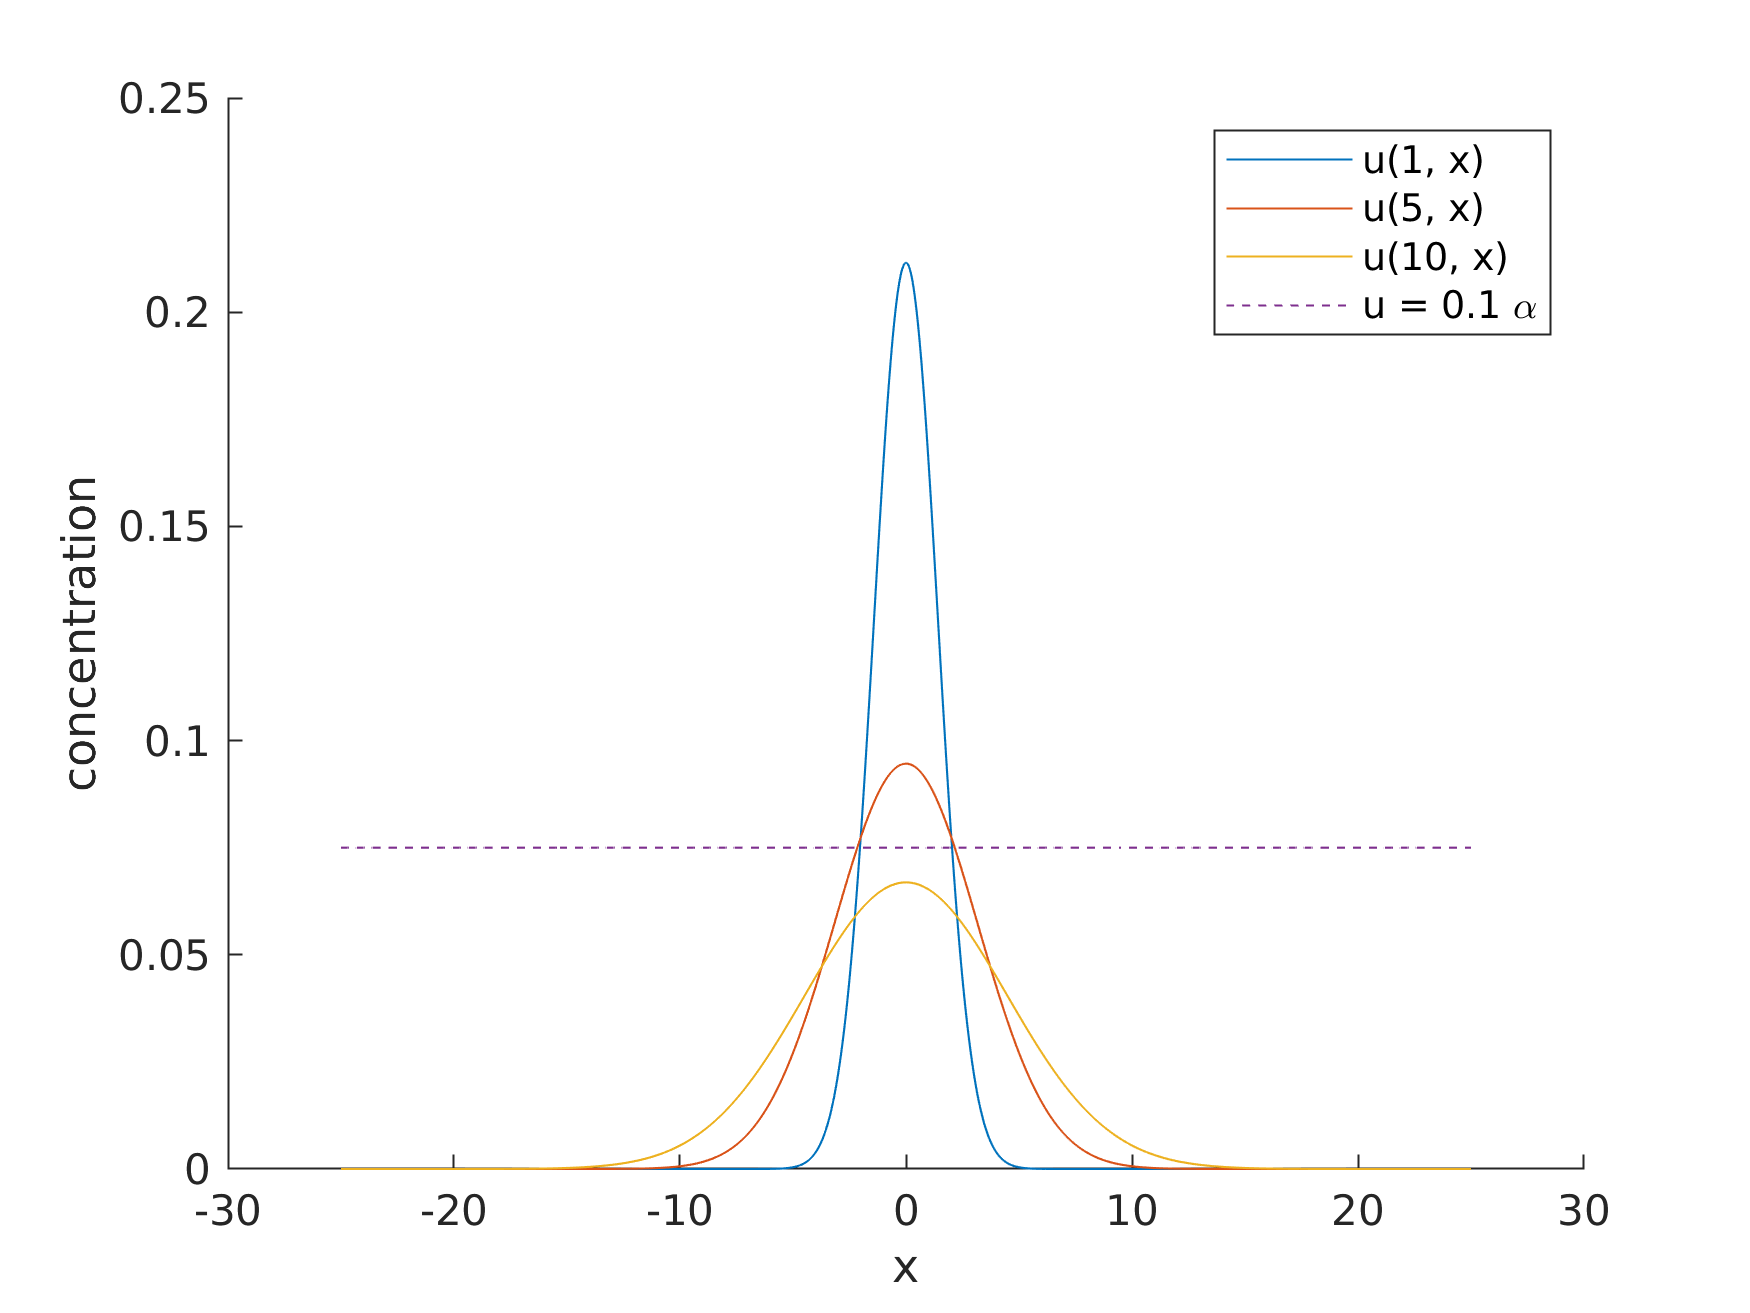
\includegraphics[width=5in]{q453a}
    \centering
    \caption{Plot of $u(t, x)$ for different times $t$ and $\alpha = 0.75$}
    \label{fig:q453a}
\end{figure}

For each point $(t_0, x_0)$, if an ant were to react to a stimulus
we would require that $u(t_0, x_0) \geq 0.1 \alpha$. Simplifying this
constraint, we have
%
\begin{align*}
    &\frac{\alpha}{2 \sqrt{\pi t_0}} e^{-\frac{x_0^2}{4 t_0}} \geq 0.1 \alpha \\
    &\implies \frac{5}{\sqrt{\pi t_0}} e^{-\frac{x_0^2}{4 t_0}} \geq 1 \\
    &\implies x_0^2 \leq 4 t_0 \log \del{\frac{5}{\sqrt{\pi t_0}}}
    .
\end{align*}
%
Any point $(t_0, x_0)$ satisfying this constraint is a point where an
ant would react to the pheromone.

Taking the positive root, we thus obtain the function
%
\begin{equation*}
    x(t) = 4 t \log \del{\frac{5}{\sqrt{\pi t}}}
    .
\end{equation*}

\vspace{5mm}

(b) Sketch the time evolution of $x(t)$.

\textit{Solution.}
A plot of $x(t)$ is shown in Figure~\ref{fig:q453b}.

\begin{figure}
    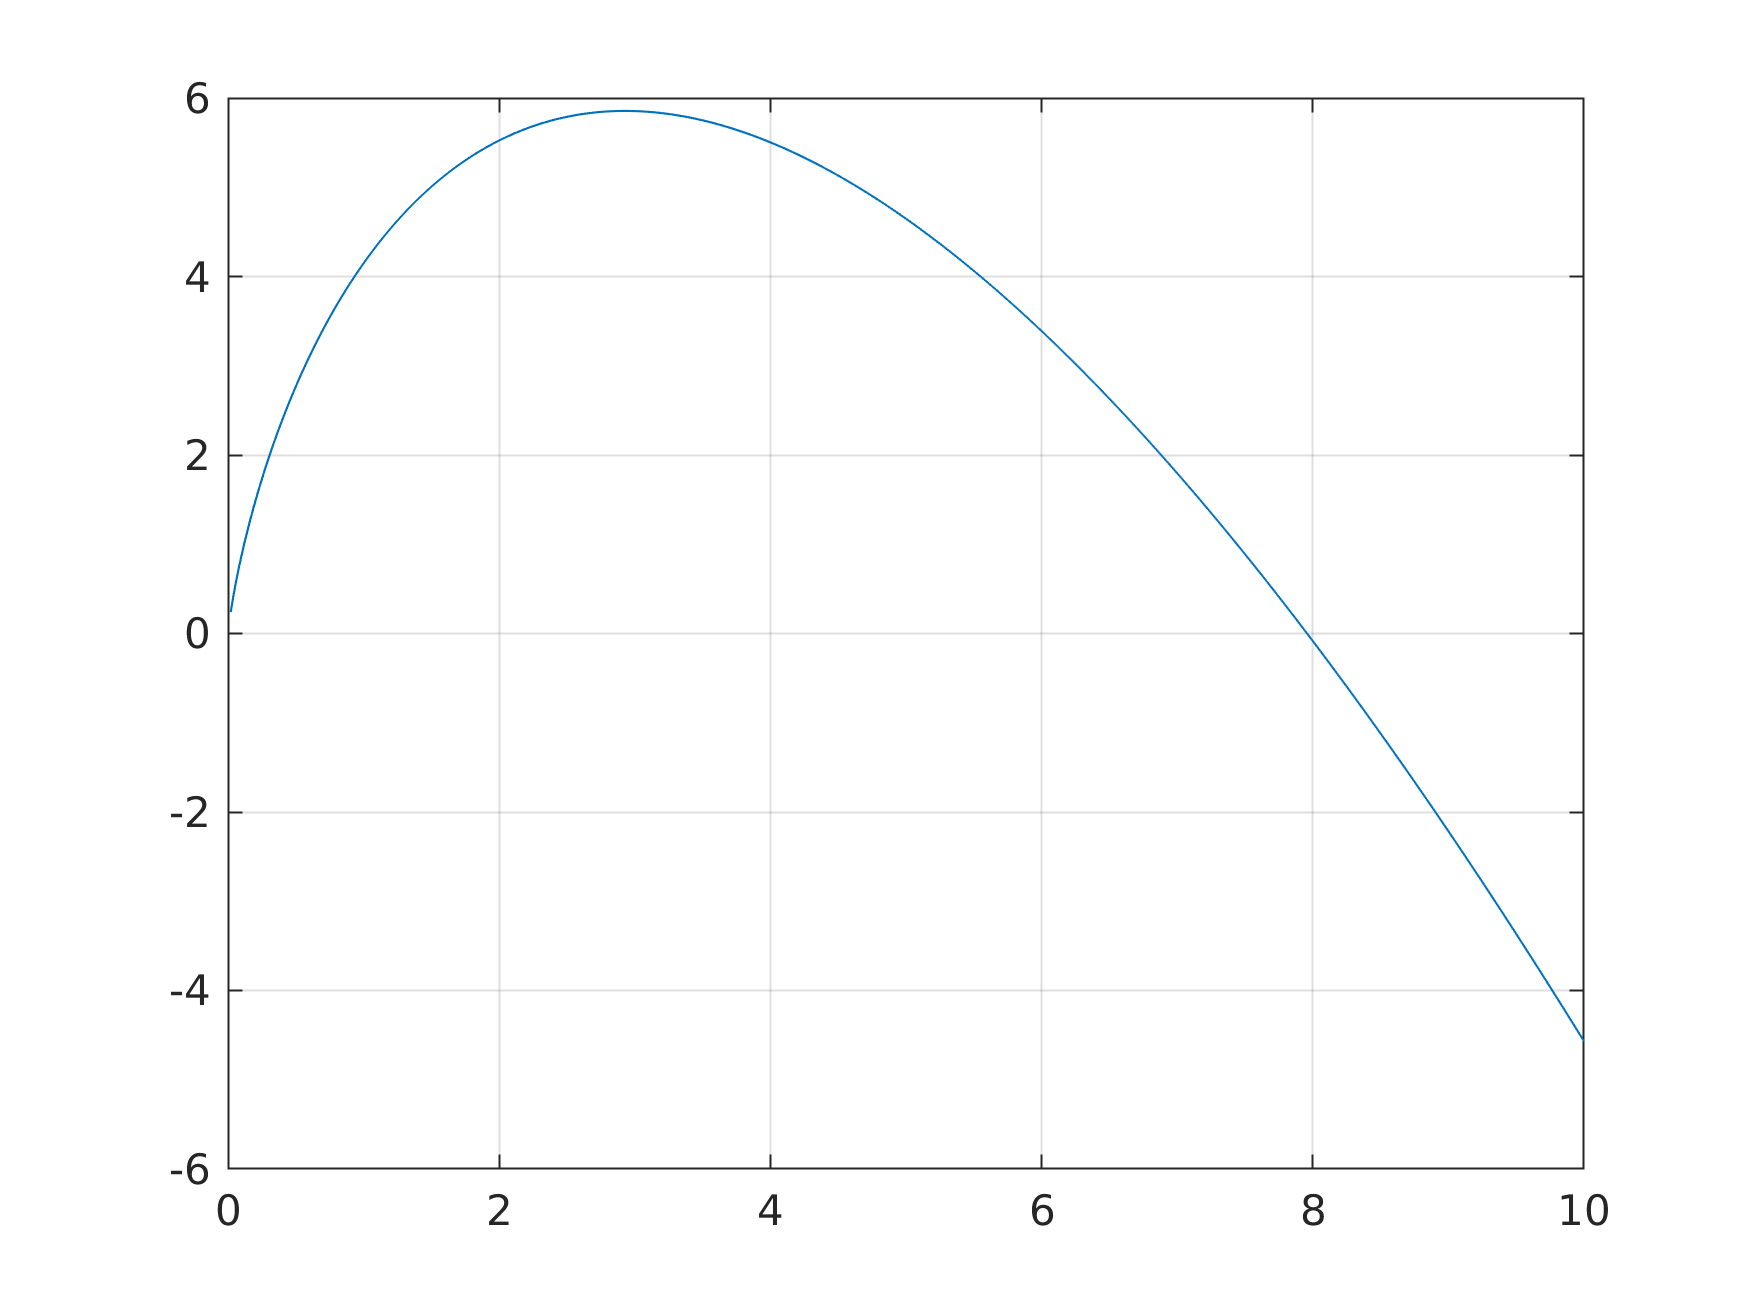
\includegraphics[width=5in]{q453b}
    \centering
    \caption{Plot of $x(t)$ from part (a)}
    \label{fig:q453b}
\end{figure}


\vspace{5mm}

(c) Find the time $t^*$ such that the region of influence is empty for all
$t > t^*$.

\textit{Solution.}
The easiest way to solve for this is to observe that $u(t, x)$ always
has its maxima in space at $x = 0$. Hence, finding $t^*$ is as simple
as solving for $u(t^*, 0) = 0.1 \alpha$:
%
\begin{align*}
    &u(t^*, 0) = 0.1 \alpha \\
    &\implies \frac{\alpha}{2 \sqrt{\pi t^*}} e^0 = 0.1 \alpha \\
    &\implies \frac{5}{\sqrt{\pi t^*}} = 1 \\
    &\implies t^* = \frac{25}{\pi}
    .
\end{align*}

\newpage

5.8.2. Use Table 5.2 (from the course textbook) and show that the eigenvector
$u^*$ of the transition matrix $P$ with eigenvalue $1$ is given by formula 5.3
(also from the course textbook).

\textit{Solution.}
Following the notation used in the course textbook, the columns of the
probability vector are, in order, RO, HI, TU, RM, BE. We will relabel
these as $o$, $h$, $t$, $m$, and $b$, respectively. The associated
transition matrix $P$ is then given by
%
\begin{equation*}
    P =
    \begin{pmatrix}
        0.12 & 0.14 & 0.12 & 0.12 & 0.13 \\
        0.12 & 0.05 & 0.08 & 0.28 & 0.27 \\
        0.12 & 0.10 & 0.10 & 0.05 & 0.08 \\
        0.42 & 0.53 & 0.32 & 0.20 & 0.19 \\
        0.22 & 0.18 & 0.38 & 0.35 & 0.33
    \end{pmatrix}
    .
\end{equation*}
%
To obtain the eigenvector $u^*$, we find the solution of
%
\begin{equation*}
    (P - I) u^* = 0
    \implies
    \begin{pmatrix}
        - 0.88 & 0.14 & 0.12 & 0.12 & 0.13 \\
        0.12 & - 0.95 & 0.08 & 0.28 & 0.27 \\
        0.12 & 0.10 & - 0.90 & 0.05 & 0.08 \\
        0.42 & 0.53 & 0.32 & - 0.80 & 0.19 \\
        0.22 & 0.18 & 0.38 & 0.35 & - 0.67
    \end{pmatrix}
    \begin{pmatrix}
        o^* \\
        h^* \\
        t^* \\
        m^* \\
        b^*
    \end{pmatrix}
    = 0
    %
\end{equation*}
%
where the columns of $u^*$ sum to $1$.
Equivalently, we can obtain $u^*$ by solving
%
\begin{align*}
    - 0.88 o^* + 0.14 h^* + 0.12 t^* + 0.12 m^* + 0.13 b^* &= 0, \\
    0.12 o^* - 0.95  h^* + 0.08 t^* + 0.28 m^* + 0.27 b^* &= 0, \\
    0.12 o^* + 0.10  h^* - 0.90 t^* + 0.05 m^* + 0.08 b^* &= 0, \\
    0.42 o^* + 0.53  h^* + 0.32 t^* - 0.80 m^* + 0.19 b^* &= 0, \\
    0.22 o^* + 0.18  h^* + 0.38 t^* + 0.35 m^* - 0.67 b^* &= 0,
\end{align*}
and then normalizing to ensure that all variables sum to $1$. Solving
this system of equations in Maple, we obtain
%
\begin{align*}
    o^* &= 1.554108928 x, \\
    h^* &= 2.394060124 x, \\
    t^* &= x, \\
    m^* &= 3.665379365 x, \\
    b^* &= 3.635399350 x,
    .
\end{align*}
%
To determine what $x$ should be, we solve
%
\begin{align*}
    &1.554108928 x + 2.394060124 x + x + 3.665379365 x + 3.635399350 x = 1 \\
    &\implies 12.24894777 x = 1 \\
    &\implies x = 0.08163966561
    .
\end{align*}
%
Hence we obtain the approximate (due to floating point arithmetic)
solution
%
\begin{align*}
    o^* &= 0.1268769332, \\
    h^* &= 0.1954502680, \\
    t^* &= 0.0816396656, \\
    m^* &= 0.2992403457, \\
    b^* &= 0.2967927873,
    .
\end{align*}
%
which agrees closely with the solution in the course textbook (which
itself is an approximate solution).

\end{document}
